\chapter{Programación dinámica}

\index{programación dinámica}

\key{Programación dinámica}
es una técnica que combina la correctitud
de la búsqueda completa y la eficiencia
de los algoritmos voraces.
La programación dinámica se puede aplicar si el
problema se puede dividir en subproblemas superpuestos
que se pueden resolver de forma independiente.

Hay dos usos para la programación dinámica:

\begin{itemize}
\item
\key{Encontrar una solución óptima}:
Queremos encontrar una solución que sea
lo más grande posible o lo más pequeña posible.
\item
\key{Contar el número de soluciones}:
Queremos calcular el número total de
soluciones posibles.
\end{itemize}

Primero veremos cómo la programación dinámica puede
usarse para encontrar una solución óptima,
y luego usaremos la misma idea para
contar las soluciones.

Entender la programación dinámica es un hito
en la carrera de todo programador competitivo.
Si bien la idea básica es simple,
el desafío es cómo aplicar
la programación dinámica a diferentes problemas.
Este capítulo presenta un conjunto de problemas clásicos
que son un buen punto de partida.

\section{Problema de las monedas}

Primero nos enfocamos en un problema que ya
hemos visto en el Capítulo 6:
Dado un conjunto de valores de monedas $\texttt{monedas} = \{c_1,c_2,\ldots,c_k\}$
y una suma objetivo de dinero $n$, nuestra tarea es
formar la suma $n$ usando la menor cantidad de monedas posible.

En el Capítulo 6, resolvimos el problema usando un
algoritmo voraz que siempre elige la moneda
más grande posible.
El algoritmo voraz funciona, por ejemplo,
cuando las monedas son las monedas de euro,
pero en el caso general, el algoritmo voraz
no necesariamente produce una solución óptima.

Ahora es el momento de resolver el problema de manera eficiente
usando programación dinámica, de modo que el algoritmo
funcione para cualquier conjunto de monedas.
El algoritmo de programación dinámica
se basa en una función recursiva
que analiza todas las posibilidades de cómo
formar la suma, como un algoritmo de fuerza bruta.
Sin embargo, el algoritmo de programación dinámica
es eficiente porque
utiliza \emph{memoización} y
calcula la respuesta a cada subproblema solo una vez.

\subsubsection{Formulación recursiva}

La idea en la programación dinámica es
formular el problema de manera recursiva para que
la solución al problema se pueda
calcular a partir de soluciones a problemas
más pequeños.
En el problema de las monedas, un problema recursivo
natural es el siguiente:
¿cuál es el menor número de monedas
requeridas para formar una suma $x$?

Denotemos $\texttt{resolver}(x)$
como el mínimo
número de monedas requeridas para una suma $x$.
Los valores de la función dependen de los
valores de las monedas.
Por ejemplo, si $\texttt{monedas} = \{1,3,4\}$,
los primeros valores de la función son los siguientes:

\[
\begin{array}{lcl}
\texttt{resolver}(0) & = & 0 \\
\texttt{resolver}(1) & = & 1 \\
\texttt{resolver}(2) & = & 2 \\
\texttt{resolver}(3) & = & 1 \\
\texttt{resolver}(4) & = & 1 \\
\texttt{resolver}(5) & = & 2 \\
\texttt{resolver}(6) & = & 2 \\
\texttt{resolver}(7) & = & 2 \\
\texttt{resolver}(8) & = & 2 \\
\texttt{resolver}(9) & = & 3 \\
\texttt{resolver}(10) & = & 3 \\
\end{array}
\]

Por ejemplo, $\texttt{resolver}(10)=3$,
porque se necesitan al menos 3 monedas
para formar la suma 10.
La solución óptima es $3+3+4=10$.

La propiedad esencial de $\texttt{resolver}$ es
que sus valores se pueden
calcular recursivamente a partir de sus valores más pequeños.
La idea es centrarse en la \emph{primera}
moneda que elegimos para la suma.
Por ejemplo, en el escenario anterior,
la primera moneda puede ser 1, 3 o 4.
Si primero elegimos la moneda 1,
la tarea restante es formar la suma 9
usando el mínimo número de monedas,
lo cual es un subproblema del problema original.
Por supuesto, lo mismo se aplica a las monedas 3 y 4.
Así, podemos usar la siguiente fórmula recursiva
para calcular el mínimo número de monedas:
\begin{equation*}
\begin{split}
\texttt{resolver}(x) = \min( & \texttt{resolver}(x-1)+1, \\
                           & \texttt{resolver}(x-3)+1, \\
                           & \texttt{resolver}(x-4)+1).
\end{split}
\end{equation*}
El caso base de la recursión es $\texttt{resolver}(0)=0$,
porque no se necesitan monedas para formar una suma vacía.
Por ejemplo,
\[ \texttt{resolver}(10) = \texttt{resolver}(7)+1 = \texttt{resolver}(4)+2 = \texttt{resolver}(0)+3 = 3.\]

Ahora estamos listos para dar una función recursiva general
que calcule el mínimo número de
monedas necesarias para formar una suma $x$:
\begin{equation*}
    \texttt{resolver}(x) = \begin{cases}
               \infty               & x < 0\\
               0               & x = 0\\
               \min_{c \in \texttt{monedas}} \texttt{resolver}(x-c)+1 & x > 0 \\
           \end{cases}
\end{equation*}

Primero, si $x<0$, el valor es $\infty$,
porque es imposible formar una suma
negativa de dinero.
Luego, si $x=0$, el valor es $0$,
porque no se necesitan monedas para formar una suma vacía.
Finalmente, si $x>0$, la variable $c$ recorre
todas las posibilidades de cómo elegir la primera moneda
de la suma.

Una vez que se encuentra una función recursiva que resuelve el problema,
podemos implementar directamente una solución en C++
(la constante \texttt{INF} denota infinito):

\begin{lstlisting}
int resolver(int x) {
    if (x < 0) return INF;
    if (x == 0) return 0;
    int mejor = INF;
    for (auto c : monedas) {
        mejor = min(mejor, resolver(x-c)+1);
    }
    return mejor;
}
\end{lstlisting}

Sin embargo, esta función no es eficiente,
porque puede haber un número exponencial de formas
de construir la suma.
No obstante, a continuación veremos cómo hacer que la
función sea eficiente utilizando una técnica llamada memoización.

\subsubsection{Usando memoización}

\index{memoización}

La idea de la programación dinámica es utilizar
\key{memoización} para calcular eficientemente
los valores de una función recursiva.
Esto significa que los valores de la función
se almacenan en un arreglo después de calcularlos.
Para cada parámetro, el valor de la función
se calcula recursivamente solo una vez y, después de esto,
el valor se puede recuperar directamente del arreglo.

En este problema, usamos los arreglos
\begin{lstlisting}
bool listo[N];
int valor[N];
\end{lstlisting}

donde $\texttt{listo}[x]$ indica
si se ha calculado el valor de $\texttt{resolver}(x)$,
y si lo está, $\texttt{valor}[x]$
contiene este valor.
La constante $N$ se ha elegido de manera que
todos los valores requeridos quepan en los arreglos.

Ahora la función se puede implementar de manera eficiente de la siguiente forma:

\begin{lstlisting}
int resolver(int x) {
    if (x < 0) return INF;
    if (x == 0) return 0;
    if (listo[x]) return valor[x];
    int mejor = INF;
    for (auto c : monedas) {
        mejor = min(mejor, resolver(x-c)+1);
    }
    valor[x] = mejor;
    listo[x] = true;
    return mejor;
}
\end{lstlisting}

La función maneja los casos base
$x<0$ y $x=0$ como antes.
Luego, la función verifica en
$\texttt{listo}[x]$ si
$\texttt{resolver}(x)$ ya ha sido almacenado
en $\texttt{valor}[x]$,
y si es así, la función lo devuelve directamente.
De lo contrario, la función calcula el valor
de $\texttt{resolver}(x)$
recursivamente y lo almacena en $\texttt{valor}[x]$.

Esta función funciona de manera eficiente,
porque la respuesta para cada parámetro $x$
se calcula recursivamente solo una vez.
Después de que se haya almacenado un valor de $\texttt{resolver}(x)$ en $\texttt{valor}[x]$,
se puede recuperar de manera eficiente cada vez que
la función sea llamada nuevamente con el parámetro $x$.
La complejidad en tiempo del algoritmo es $O(nk)$,
donde $n$ es la suma objetivo y $k$ es el número de monedas.

También podemos construir \emph{iterativamente}
el arreglo \texttt{valor} usando
un bucle que simplemente calcule todos los valores
de $\texttt{resolver}$ para los parámetros $0 \ldots n$:
\begin{lstlisting}
valor[0] = 0;
for (int x = 1; x <= n; x++) {
    valor[x] = INF;
    for (auto c : monedas) {
        if (x-c >= 0) {
            valor[x] = min(valor[x], valor[x-c]+1);
        }
    }
}
\end{lstlisting}

De hecho, la mayoría de los programadores competitivos prefieren esta
implementación, porque es más corta y tiene
factores constantes más bajos.
A partir de ahora, también utilizamos implementaciones iterativas
en nuestros ejemplos.
Aun así, a menudo es más fácil pensar en soluciones
de programación dinámica
en términos de funciones recursivas.


\subsubsection{Construyendo una solución}

A veces se nos pide encontrar el valor
de una solución óptima y dar
un ejemplo de cómo se puede construir dicha solución.
En el problema de las monedas, por ejemplo,
podemos declarar otro arreglo
que indique para
cada suma de dinero la primera moneda
en una solución óptima:
\begin{lstlisting}
int primero[N];
\end{lstlisting}
Luego, podemos modificar el algoritmo de la siguiente manera:
\begin{lstlisting}
valor[0] = 0;
for (int x = 1; x <= n; x++) {
    valor[x] = INF;
    for (auto c : monedas) {
        if (x-c >= 0 && valor[x-c]+1 < valor[x]) {
            valor[x] = valor[x-c]+1;
            primero[x] = c;
        }
    }
}
\end{lstlisting}
Después de esto, el siguiente código se puede utilizar para
imprimir las monedas que aparecen en una solución óptima para
la suma $n$:
\begin{lstlisting}
while (n > 0) {
    cout << primero[n] << "\n";
    n -= primero[n];
}
\end{lstlisting}

\subsubsection{Contando el número de soluciones}

Ahora consideremos otra versión
del problema de las monedas donde nuestra tarea es
calcular el número total de formas
de obtener una suma $x$ usando las monedas.
Por ejemplo, si $\texttt{monedas}=\{1,3,4\}$ y
$x=5$, hay un total de 6 formas:

\begin{multicols}{2}
\begin{itemize}
\item $1+1+1+1+1$
\item $1+1+3$
\item $1+3+1$
\item $3+1+1$
\item $1+4$
\item $4+1$
\end{itemize}
\end{multicols}

De nuevo, podemos resolver el problema recursivamente.
Sea $\texttt{resolver}(x)$ el número de formas
en las que podemos formar la suma $x$.
Por ejemplo, si $\texttt{monedas}=\{1,3,4\}$,
entonces $\texttt{resolver}(5)=6$ y la fórmula recursiva es
\begin{equation*}
\begin{split}
\texttt{resolver}(x) = & \texttt{resolver}(x-1) + \\
                    & \texttt{resolver}(x-3) + \\
                    & \texttt{resolver}(x-4)  .
\end{split}
\end{equation*}

Entonces, la función recursiva general es la siguiente:
\begin{equation*}
    \texttt{resolver}(x) = \begin{cases}
               0               & x < 0\\
               1               & x = 0\\
               \sum_{c \in \texttt{monedas}} \texttt{resolver}(x-c) & x > 0 \\
           \end{cases}
\end{equation*}

Si $x<0$, el valor es 0, porque no hay soluciones.
Si $x=0$, el valor es 1, porque solo hay una forma
de formar una suma vacía.
De lo contrario, calculamos la suma de todos los valores
de la forma $\texttt{resolver}(x-c)$ donde $c$ está en \texttt{monedas}.

El siguiente código construye un array
$\texttt{conteo}$ tal que
$\texttt{conteo}[x]$ es igual
al valor de $\texttt{resolver}(x)$
para $0 \le x \le n$:

\begin{lstlisting}
conteo[0] = 1;
for (int x = 1; x <= n; x++) {
    for (auto c : monedas) {
        if (x-c >= 0) {
            conteo[x] += conteo[x-c];
        }
    }
}
\end{lstlisting}

A menudo, el número de soluciones es tan grande
que no es necesario calcular el número exacto
pero es suficiente dar la respuesta módulo $m$
donde, por ejemplo, $m=10^9+7$.
Esto se puede hacer modificando el código de manera que
todos los cálculos se realicen módulo $m$.
En el código anterior, basta con agregar la línea
\begin{lstlisting}
        conteo[x] %= m;
\end{lstlisting}
después de la línea
\begin{lstlisting}
        conteo[x] += conteo[x-c];
\end{lstlisting}

Ahora hemos discutido todas las ideas básicas
de la programación dinámica.
Dado que la programación dinámica se puede utilizar
en muchas situaciones diferentes,
ahora revisaremos un conjunto de problemas
que muestran más ejemplos sobre las
posibilidades de la programación dinámica.

\section{Subsecuencia creciente más larga}

\index{subsecuencia creciente más larga}

Nuestro primer problema es encontrar la
\key{subsecuencia creciente más larga}
en un arreglo de $n$ elementos.
Esta es una secuencia de longitud máxima
de elementos del arreglo
que va de izquierda a derecha,
y cada elemento en la secuencia es mayor
que el elemento anterior.
Por ejemplo, en el arreglo

\begin{center}
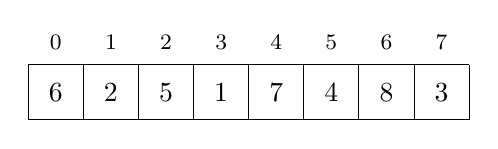
\begin{tikzpicture}[scale=0.7]
\draw (0,0) grid (8,1);
\node at (0.5,0.5) {$6$};
\node at (1.5,0.5) {$2$};
\node at (2.5,0.5) {$5$};
\node at (3.5,0.5) {$1$};
\node at (4.5,0.5) {$7$};
\node at (5.5,0.5) {$4$};
\node at (6.5,0.5) {$8$};
\node at (7.5,0.5) {$3$};

\footnotesize
\node at (0.5,1.4) {$0$};
\node at (1.5,1.4) {$1$};
\node at (2.5,1.4) {$2$};
\node at (3.5,1.4) {$3$};
\node at (4.5,1.4) {$4$};
\node at (5.5,1.4) {$5$};
\node at (6.5,1.4) {$6$};
\node at (7.5,1.4) {$7$};
\end{tikzpicture}
\end{center}
la subsecuencia creciente más larga
contiene 4 elementos:
\begin{center}
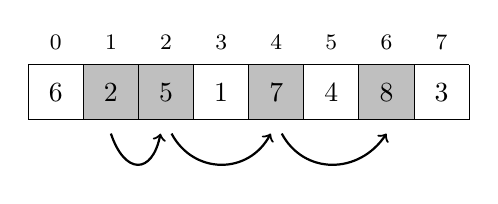
\begin{tikzpicture}[scale=0.7]
\fill[color=lightgray] (1,0) rectangle (2,1);
\fill[color=lightgray] (2,0) rectangle (3,1);
\fill[color=lightgray] (4,0) rectangle (5,1);
\fill[color=lightgray] (6,0) rectangle (7,1);
\draw (0,0) grid (8,1);
\node at (0.5,0.5) {$6$};
\node at (1.5,0.5) {$2$};
\node at (2.5,0.5) {$5$};
\node at (3.5,0.5) {$1$};
\node at (4.5,0.5) {$7$};
\node at (5.5,0.5) {$4$};
\node at (6.5,0.5) {$8$};
\node at (7.5,0.5) {$3$};

\draw[thick,->] (1.5,-0.25) .. controls (1.75,-1.00) and (2.25,-1.00) .. (2.4,-0.25);
\draw[thick,->] (2.6,-0.25) .. controls (3.0,-1.00) and (4.0,-1.00) .. (4.4,-0.25);
\draw[thick,->] (4.6,-0.25) .. controls (5.0,-1.00) and (6.0,-1.00) .. (6.5,-0.25);

\footnotesize
\node at (0.5,1.4) {$0$};
\node at (1.5,1.4) {$1$};
\node at (2.5,1.4) {$2$};
\node at (3.5,1.4) {$3$};
\node at (4.5,1.4) {$4$};
\node at (5.5,1.4) {$5$};
\node at (6.5,1.4) {$6$};
\node at (7.5,1.4) {$7$};
\end{tikzpicture}
\end{center}

Denotemos $\texttt{largo}(k)$ como
el largo de la
subsecuencia creciente más larga
que termina en la posición $k$.
Así, si calculamos todos los valores de
$\texttt{largo}(k)$ donde $0 \le k \le n-1$,
descubriremos el largo de la
subsecuencia creciente más larga.
Por ejemplo, los valores de la función
para el arreglo anterior son los siguientes:
\[
\begin{array}{lcl}
\texttt{largo}(0) & = & 1 \\
\texttt{largo}(1) & = & 1 \\
\texttt{largo}(2) & = & 2 \\
\texttt{largo}(3) & = & 1 \\
\texttt{largo}(4) & = & 3 \\
\texttt{largo}(5) & = & 2 \\
\texttt{largo}(6) & = & 4 \\
\texttt{largo}(7) & = & 2 \\
\end{array}
\]

Por ejemplo, $\texttt{largo}(6)=4$,
porque la subsecuencia creciente más larga
que termina en la posición 6 consta de 4 elementos.

Para calcular un valor de $\texttt{largo}(k)$,
debemos encontrar una posición $i<k$
tal que $\texttt{arreglo}[i]<\texttt{arreglo}[k]$
y $\texttt{largo}(i)$ sea lo más grande posible.
Entonces sabemos que
$\texttt{largo}(k)=\texttt{largo}(i)+1$,
porque esta es una forma óptima de agregar
$\texttt{arreglo}[k]$ a una subsecuencia.
Sin embargo, si no existe tal posición $i$,
entonces $\texttt{largo}(k)=1$,
lo que significa que la subsecuencia solo contiene
$\texttt{arreglo}[k]$.

Dado que todos los valores de la función se pueden calcular
a partir de sus valores más pequeños,
podemos utilizar la programación dinámica.
En el siguiente código, los valores
de la función se almacenarán en un arreglo
$\texttt{largo}$.

\begin{lstlisting}
for (int k = 0; k < n; k++) {
    largo[k] = 1;
    for (int i = 0; i < k; i++) {
        if (arreglo[i] < arreglo[k]) {
            largo[k] = max(largo[k],largo[i]+1);
        }
    }
}
\end{lstlisting}

Este código funciona en tiempo $O(n^2)$,
porque consta de dos bucles anidados.
Sin embargo, también es posible implementar
el cálculo de programación dinámica
de manera más eficiente en tiempo $O(n \log n)$.
¿Puedes encontrar una forma de hacer esto?

\section{Caminos en una cuadrícula}

Nuestro siguiente problema es encontrar un camino
desde la esquina superior izquierda hasta
la esquina inferior derecha
de una cuadrícula de $n \times n$, de tal manera que
sólo nos movemos hacia abajo y hacia la derecha.
Cada cuadro contiene un número entero positivo,
y el camino debe construirse de tal manera que
la suma de los valores a lo largo
del camino sea lo más grande posible.

La siguiente imagen muestra un camino óptimo
en una cuadrícula:
\begin{center}
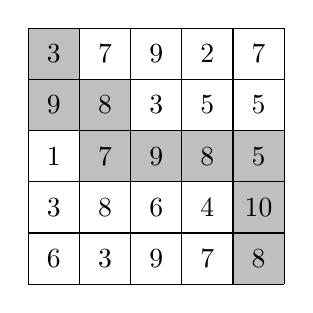
\begin{tikzpicture}[scale=.65]
  \begin{scope}
    \fill [color=lightgray] (0, 9) rectangle (1, 8);
    \fill [color=lightgray] (0, 8) rectangle (1, 7);
    \fill [color=lightgray] (1, 8) rectangle (2, 7);
    \fill [color=lightgray] (1, 7) rectangle (2, 6);
    \fill [color=lightgray] (2, 7) rectangle (3, 6);
    \fill [color=lightgray] (3, 7) rectangle (4, 6);
    \fill [color=lightgray] (4, 7) rectangle (5, 6);
    \fill [color=lightgray] (4, 6) rectangle (5, 5);
    \fill [color=lightgray] (4, 5) rectangle (5, 4);
    \draw (0, 4) grid (5, 9);
    \node at (0.5,8.5) {3};
    \node at (1.5,8.5) {7};
    \node at (2.5,8.5) {9};
    \node at (3.5,8.5) {2};
    \node at (4.5,8.5) {7};
    \node at (0.5,7.5) {9};
    \node at (1.5,7.5) {8};
    \node at (2.5,7.5) {3};
    \node at (3.5,7.5) {5};
    \node at (4.5,7.5) {5};
    \node at (0.5,6.5) {1};
    \node at (1.5,6.5) {7};
    \node at (2.5,6.5) {9};
    \node at (3.5,6.5) {8};
    \node at (4.5,6.5) {5};
    \node at (0.5,5.5) {3};
    \node at (1.5,5.5) {8};
    \node at (2.5,5.5) {6};
    \node at (3.5,5.5) {4};
    \node at (4.5,5.5) {10};
    \node at (0.5,4.5) {6};
    \node at (1.5,4.5) {3};
    \node at (2.5,4.5) {9};
    \node at (3.5,4.5) {7};
    \node at (4.5,4.5) {8};
  \end{scope}
\end{tikzpicture}
\end{center}
La suma de los valores en el camino es 67,
y esta es la suma más grande posible en un camino
desde la esquina
superior izquierda hasta la esquina inferior derecha.

Suponga que las filas y columnas de la
cuadrícula están numeradas del 1 al $n$,
y $\texttt{valor}[y][x]$ es igual al valor
del cuadro $(y,x)$.
Sea $\texttt{suma}(y,x)$ la suma máxima
en un camino desde la esquina superior izquierda
hasta el cuadro $(y,x)$.
Ahora, $\texttt{suma}(n,n)$ nos indica
la suma máxima
desde la esquina superior izquierda hasta
la esquina inferior derecha.
Por ejemplo, en la cuadrícula anterior,
$\texttt{suma}(5,5)=67$.

Podemos calcular recursivamente las sumas
de la siguiente manera:
\[ \texttt{suma}(y,x) = \max(\texttt{suma}(y,x-1),\texttt{suma}(y-1,x))+\texttt{valor}[y][x]\]

La fórmula recursiva se basa en la observación
de que un camino que termina en el cuadro $(y,x)$
puede provenir del cuadro $(y,x-1)$
o del cuadro $(y-1,x)$:
\begin{center}
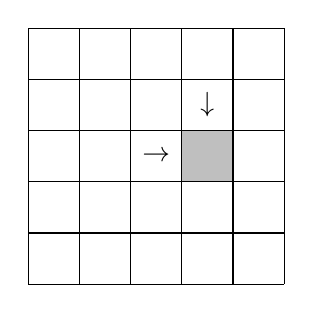
\begin{tikzpicture}[scale=.65]
  \begin{scope}
    \fill [color=lightgray] (3, 7) rectangle (4, 6);
    \draw (0, 4) grid (5, 9);
    
    \node at (2.5,6.5) {$\rightarrow$};
    \node at (3.5,7.5) {$\downarrow$};
    
  \end{scope}
\end{tikzpicture}
\end{center}

Por lo tanto, seleccionamos la dirección que maximiza
la suma.
Asumimos que $\texttt{suma}(y,x)=0$
si $y=0$ o $x=0$ (porque no existen tales caminos),
así que la fórmula recursiva también funciona cuando $y=1$ o $x=1$.

Dado que la función \texttt{suma} tiene dos parámetros,
el array de programación dinámica también tiene dos dimensiones.
Por ejemplo, podemos usar un array
\begin{lstlisting}
int suma[N][N];
\end{lstlisting}
y calcular la suma como sigue:
\begin{lstlisting}
for (int y = 1; y <= n; y++) {
    for (int x = 1; x <= n; x++) {
        suma[y][x] = max(suma[y][x-1],suma[y-1][x])+valor[y][x];
    }
}
\end{lstlisting}
La complejidad temporal del algoritmo es $O(n^2)$.

\section{Problemas de la mochila}

\index{mochila}

El término \key{mochila} se refiere a problemas donde
se da un conjunto de objetos y
se deben encontrar subconjuntos con ciertas propiedades.
Los problemas de la mochila a menudo se pueden resolver
usando programación dinámica.

En esta sección, nos enfocamos en el siguiente
problema: Dada una lista de pesos
$[w_1,w_2,\ldots,w_n]$,
determine todas
las sumas que se pueden construir usando los pesos.
Por ejemplo, si los pesos son
$[1,3,3,5]$, las siguientes sumas son posibles:

\begin{center}
\begin{tabular}{rrrrrrrrrrrrr}
 0 & 1 & 2 & 3 & 4 & 5 & 6 & 7 & 8 & 9 & 10 & 11 & 12 \\
\hline
 X & X & & X & X & X & X & X & X & X & & X & X \\
\end{tabular}
\end{center}

En este caso, todas las sumas entre $0 \ldots 12$
son posibles, excepto 2 y 10.
Por ejemplo, la suma 7 es posible porque podemos
seleccionar los pesos $[1,3,3]$.

Para resolver el problema, nos enfocamos en subproblemas
donde solo usamos los primeros $k$ pesos
para construir sumas.
Sea $\texttt{posible}(x,k)=\textrm{verdadero}$ si
podemos construir una suma $x$
usando los primeros $k$ pesos,
y de lo contrario $\texttt{posible}(x,k)=\textrm{falso}$.
Los valores de la función se pueden calcular recursivamente de la siguiente manera:
\[ \texttt{posible}(x,k) = \texttt{posible}(x-w_k,k-1) \lor \texttt{posible}(x,k-1) \]
La fórmula se basa en el hecho de que podemos
usar o no usar el peso $w_k$ en la suma.
Si usamos $w_k$, la tarea restante es formar
la suma $x-w_k$ usando los primeros $k-1$ pesos,
y si no usamos $w_k$,
la tarea restante es formar la suma $x$
usando los primeros $k-1$ pesos.
Como casos base,
\begin{equation*}
    \texttt{posible}(x,0) = \begin{cases}
               \textrm{verdadero}    & x = 0\\
               \textrm{falso}   & x \neq 0 \\
           \end{cases}
\end{equation*}
porque si no se usan pesos,
solo podemos formar la suma 0.

La siguiente tabla muestra todos los valores de la función
para los pesos $[1,3,3,5]$ (el símbolo "X"
indica los valores verdaderos):

\begin{center}
\begin{tabular}{r|rrrrrrrrrrrrr}
$k \backslash x$ & 0 & 1 & 2 & 3 & 4 & 5 & 6 & 7 & 8 & 9 & 10 & 11 & 12 \\
\hline
 0 & X & \\
 1 & X & X \\
 2 & X & X & & X & X \\
 3 & X & X & & X & X & & X & X \\
 4 & X & X & & X & X & X & X & X & X & X & & X & X \\
\end{tabular}
\end{center}

Después de calcular esos valores, $\texttt{posible}(x,n)$
nos indica si podemos construir una
suma $x$ utilizando \emph{todos} los pesos.

Denotemos $W$ como la suma total de los pesos.
La siguiente solución de programación dinámica $O(nW)$
corresponde a la función recursiva:
\begin{lstlisting}
posible[0][0] = true;
for (int k = 1; k <= n; k++) {
    for (int x = 0; x <= W; x++) {
        if (x-w[k] >= 0) posible[x][k] |= posible[x-w[k]][k-1];
        posible[x][k] |= posible[x][k-1];
    }
}
\end{lstlisting}

Sin embargo, aquí hay una mejor implementación que solo utiliza
un arreglo unidimensional $\texttt{posible}[x]$
que indica si podemos construir un subconjunto con suma $x$.
El truco es actualizar el arreglo de derecha a izquierda para
cada nuevo peso:
\begin{lstlisting}
posible[0] = true;
for (int k = 1; k <= n; k++) {
    for (int x = W; x >= 0; x--) {
        if (posible[x]) posible[x+w[k]] = true;
    }
}
\end{lstlisting}

Tenga en cuenta que la idea general presentada aquí se puede utilizar
en muchos problemas de mochila.
Por ejemplo, si se nos dan objetos con pesos y valores,
podemos determinar para cada suma de pesos el valor máximo
suma de un subconjunto.

\section{Distancia de edición}

\index{distancia de edición}
\index{distancia de Levenshtein}

La \key{distancia de edición} o \key{distancia de Levenshtein}\footnote{La distancia
lleva el nombre de V. I. Levenshtein, quien la estudió en relación con los códigos binarios \cite{lev66}.}
es el número mínimo de operaciones de edición
necesarias para transformar una cadena
en otra cadena.
Las operaciones de edición permitidas son las siguientes:
\begin{itemize}
\item insertar un carácter (por ejemplo, \texttt{ABC} $\rightarrow$ \texttt{ABCA})
\item eliminar un carácter (por ejemplo, \texttt{ABC} $\rightarrow$ \texttt{AC})
\item modificar un carácter (por ejemplo, \texttt{ABC} $\rightarrow$ \texttt{ADC})
\end{itemize}

Por ejemplo, la distancia de edición entre
\texttt{LOVE} y \texttt{MOVIE} es 2,
porque primero podemos realizar la operación
 \texttt{LOVE} $\rightarrow$ \texttt{MOVE}
(modificar) y luego la operación
\texttt{MOVE} $\rightarrow$ \texttt{MOVIE}
(insertar).
Este es el número mínimo posible de operaciones,
porque está claro que una sola operación no es suficiente.

Supongamos que se nos da una cadena \texttt{x}
de longitud $n$ y una cadena \texttt{y} de longitud $m$,
y queremos calcular la distancia de edición entre
\texttt{x} y \texttt{y}.
Para resolver el problema, definimos una función
$\texttt{distancia}(a,b)$ that gives the
edit distance between prefixes
$\texttt{x}[0 \ldots a]$ and $\texttt{y}[0 \ldots b]$.
Thus, using this function, the edit distance
between \texttt{x} and \texttt{y} equals $\texttt{distance}(n-1,m-1)$.

We can calculate values of \texttt{distance}
as follows:
\begin{equation*}
\begin{split}
\texttt{distance}(a,b) = \min(& \texttt{distance}(a,b-1)+1, \\
                           & \texttt{distance}(a-1,b)+1, \\
                           & \texttt{distance}(a-1,b-1)+\texttt{cost}(a,b)).
\end{split}
\end{equation*}
Here $\texttt{cost}(a,b)=0$ if $\texttt{x}[a]=\texttt{y}[b]$,
and otherwise $\texttt{cost}(a,b)=1$.
The formula considers the following ways to
edit the string \texttt{x}:
\begin{itemize}
\item $\texttt{distance}(a,b-1)$: insert a character at the end of \texttt{x}
\item $\texttt{distance}(a-1,b)$: remove the last character from \texttt{x}
\item $\texttt{distance}(a-1,b-1)$: match or modify the last character of \texttt{x}
\end{itemize}
In the two first cases, one editing operation is needed
(insert or remove).
In the last case, if $\texttt{x}[a]=\texttt{y}[b]$,
we can match the last characters without editing,
and otherwise one editing operation is needed (modify).

The following table shows the values of \texttt{distance}
in the example case:
\begin{center}
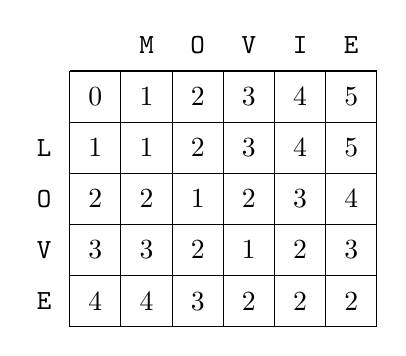
\begin{tikzpicture}[scale=.65]
  \begin{scope}
    %\fill [color=lightgray] (5, -3) rectangle (6, -4);
    \draw (1, -1) grid (7, -6);
    
    \node at (0.5,-2.5) {\texttt{L}};
    \node at (0.5,-3.5) {\texttt{O}};
    \node at (0.5,-4.5) {\texttt{V}};
    \node at (0.5,-5.5) {\texttt{E}};

    \node at (2.5,-0.5) {\texttt{M}};
    \node at (3.5,-0.5) {\texttt{O}};
    \node at (4.5,-0.5) {\texttt{V}};
    \node at (5.5,-0.5) {\texttt{I}};
    \node at (6.5,-0.5) {\texttt{E}};

    \node at (1.5,-1.5) {$0$};
    \node at (1.5,-2.5) {$1$};
    \node at (1.5,-3.5) {$2$};
    \node at (1.5,-4.5) {$3$};
    \node at (1.5,-5.5) {$4$};
    \node at (2.5,-1.5) {$1$};
    \node at (2.5,-2.5) {$1$};
    \node at (2.5,-3.5) {$2$};
    \node at (2.5,-4.5) {$3$};
    \node at (2.5,-5.5) {$4$};
    \node at (3.5,-1.5) {$2$};
    \node at (3.5,-2.5) {$2$};
    \node at (3.5,-3.5) {$1$};
    \node at (3.5,-4.5) {$2$};
    \node at (3.5,-5.5) {$3$};
    \node at (4.5,-1.5) {$3$};
    \node at (4.5,-2.5) {$3$};
    \node at (4.5,-3.5) {$2$};
    \node at (4.5,-4.5) {$1$};
    \node at (4.5,-5.5) {$2$};
    \node at (5.5,-1.5) {$4$};
    \node at (5.5,-2.5) {$4$};
    \node at (5.5,-3.5) {$3$};
    \node at (5.5,-4.5) {$2$};
    \node at (5.5,-5.5) {$2$};
    \node at (6.5,-1.5) {$5$};
    \node at (6.5,-2.5) {$5$};
    \node at (6.5,-3.5) {$4$};
    \node at (6.5,-4.5) {$3$};
    \node at (6.5,-5.5) {$2$};
  \end{scope}
\end{tikzpicture}
\end{center}

The lower-right corner of the table
tells us that the edit distance between
\texttt{LOVE} and \texttt{MOVIE} is 2.
The table also shows how to construct
the shortest sequence of editing operations.
In this case the path is as follows:

\begin{center}
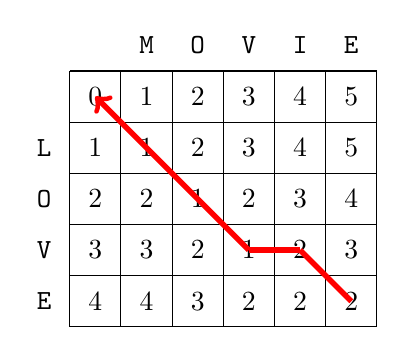
\begin{tikzpicture}[scale=.65]
  \begin{scope}
    \draw (1, -1) grid (7, -6);
    
    \node at (0.5,-2.5) {\texttt{L}};
    \node at (0.5,-3.5) {\texttt{O}};
    \node at (0.5,-4.5) {\texttt{V}};
    \node at (0.5,-5.5) {\texttt{E}};

    \node at (2.5,-0.5) {\texttt{M}};
    \node at (3.5,-0.5) {\texttt{O}};
    \node at (4.5,-0.5) {\texttt{V}};
    \node at (5.5,-0.5) {\texttt{I}};
    \node at (6.5,-0.5) {\texttt{E}};

    \node at (1.5,-1.5) {$0$};
    \node at (1.5,-2.5) {$1$};
    \node at (1.5,-3.5) {$2$};
    \node at (1.5,-4.5) {$3$};
    \node at (1.5,-5.5) {$4$};
    \node at (2.5,-1.5) {$1$};
    \node at (2.5,-2.5) {$1$};
    \node at (2.5,-3.5) {$2$};
    \node at (2.5,-4.5) {$3$};
    \node at (2.5,-5.5) {$4$};
    \node at (3.5,-1.5) {$2$};
    \node at (3.5,-2.5) {$2$};
    \node at (3.5,-3.5) {$1$};
    \node at (3.5,-4.5) {$2$};
    \node at (3.5,-5.5) {$3$};
    \node at (4.5,-1.5) {$3$};
    \node at (4.5,-2.5) {$3$};
    \node at (4.5,-3.5) {$2$};
    \node at (4.5,-4.5) {$1$};
    \node at (4.5,-5.5) {$2$};
    \node at (5.5,-1.5) {$4$};
    \node at (5.5,-2.5) {$4$};
    \node at (5.5,-3.5) {$3$};
    \node at (5.5,-4.5) {$2$};
    \node at (5.5,-5.5) {$2$};
    \node at (6.5,-1.5) {$5$};
    \node at (6.5,-2.5) {$5$};
    \node at (6.5,-3.5) {$4$};
    \node at (6.5,-4.5) {$3$};
    \node at (6.5,-5.5) {$2$};

    \path[draw=red,thick,-,line width=2pt] (6.5,-5.5) -- (5.5,-4.5);
    \path[draw=red,thick,-,line width=2pt] (5.5,-4.5) -- (4.5,-4.5);
    \path[draw=red,thick,->,line width=2pt] (4.5,-4.5) -- (1.5,-1.5);
  \end{scope}
\end{tikzpicture}
\end{center}

The last characters of \texttt{LOVE} and \texttt{MOVIE}
are equal, so the edit distance between them
equals the edit distance between \texttt{LOV} and \texttt{MOVI}.
We can use one editing operation to remove the
character \texttt{I} from \texttt{MOVI}.
Thus, the edit distance is one larger than
the edit distance between \texttt{LOV} and \texttt{MOV}, etc.

\section{Counting tilings}

Sometimes the states of a dynamic programming solution
are more complex than fixed combinations of numbers.
As an example,
consider the problem of calculating
the number of distinct ways to
fill an $n \times m$ grid using
$1 \times 2$ and $2 \times 1$ size tiles.
For example, one valid solution
for the $4 \times 7$ grid is
\begin{center}
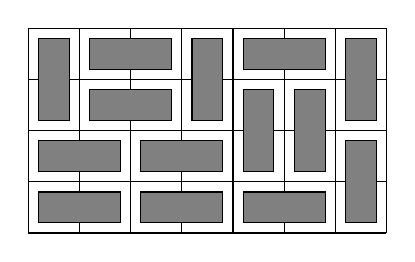
\begin{tikzpicture}[scale=.65]
    \draw (0,0) grid (7,4);
    \draw[fill=gray] (0+0.2,0+0.2) rectangle (2-0.2,1-0.2);
    \draw[fill=gray] (2+0.2,0+0.2) rectangle (4-0.2,1-0.2);
    \draw[fill=gray] (4+0.2,0+0.2) rectangle (6-0.2,1-0.2);
    \draw[fill=gray] (0+0.2,1+0.2) rectangle (2-0.2,2-0.2);
    \draw[fill=gray] (2+0.2,1+0.2) rectangle (4-0.2,2-0.2);
    \draw[fill=gray] (1+0.2,2+0.2) rectangle (3-0.2,3-0.2);
    \draw[fill=gray] (1+0.2,3+0.2) rectangle (3-0.2,4-0.2);
    \draw[fill=gray] (4+0.2,3+0.2) rectangle (6-0.2,4-0.2);

    \draw[fill=gray] (0+0.2,2+0.2) rectangle (1-0.2,4-0.2);
    \draw[fill=gray] (3+0.2,2+0.2) rectangle (4-0.2,4-0.2);
    \draw[fill=gray] (6+0.2,2+0.2) rectangle (7-0.2,4-0.2);
    \draw[fill=gray] (4+0.2,1+0.2) rectangle (5-0.2,3-0.2);
    \draw[fill=gray] (5+0.2,1+0.2) rectangle (6-0.2,3-0.2);
    \draw[fill=gray] (6+0.2,0+0.2) rectangle (7-0.2,2-0.2);

\end{tikzpicture}
\end{center}
and the total number of solutions is 781.

The problem can be solved using dynamic programming
by going through the grid row by row.
Each row in a solution can be represented as a
string that contains $m$ characters from the set
$\{\sqcap, \sqcup, \sqsubset, \sqsupset \}$.
For example, the above solution consists of four rows
that correspond to the following strings:
\begin{itemize}
\item
$\sqcap \sqsubset \sqsupset \sqcap \sqsubset \sqsupset \sqcap$
\item
$\sqcup \sqsubset \sqsupset \sqcup \sqcap \sqcap \sqcup$
\item
$\sqsubset \sqsupset \sqsubset \sqsupset \sqcup \sqcup \sqcap$ 
\item
$\sqsubset \sqsupset \sqsubset \sqsupset \sqsubset \sqsupset \sqcup$
\end{itemize}

Let $\texttt{count}(k,x)$ denote the number of ways to
construct a solution for rows $1 \ldots k$
of the grid such that string $x$ corresponds to row $k$.
It is possible to use dynamic programming here,
because the state of a row is constrained
only by the state of the previous row.

A solution is valid if row $1$ does not contain
the character $\sqcup$,
row $n$ does not contain the character $\sqcap$,
and all consecutive rows are \emph{compatible}.
For example, the rows
$\sqcup \sqsubset \sqsupset \sqcup \sqcap \sqcap \sqcup$ and
$\sqsubset \sqsupset \sqsubset \sqsupset \sqcup \sqcup \sqcap$ 
are compatible, while the rows
$\sqcap \sqsubset \sqsupset \sqcap \sqsubset \sqsupset \sqcap$ and
$\sqsubset \sqsupset \sqsubset \sqsupset \sqsubset \sqsupset \sqcup$
are not compatible.

Since a row consists of $m$ characters and there are
four choices for each character, the number of distinct
rows is at most $4^m$.
Thus, the time complexity of the solution is
$O(n 4^{2m})$ because we can go through the
$O(4^m)$ possible states for each row,
and for each state, there are $O(4^m)$
possible states for the previous row.
In practice, it is a good idea to rotate the grid
so that the shorter side has length $m$,
because the factor $4^{2m}$ dominates the time complexity.

It is possible to make the solution more efficient
by using a more compact representation for the rows.
It turns out that it is sufficient to know which
columns of the previous row contain the upper square
of a vertical tile.
Thus, we can represent a row using only characters
$\sqcap$ and $\Box$, where $\Box$ is a combination
of characters
$\sqcup$, $\sqsubset$ and $\sqsupset$.
Using this representation, there are only
$2^m$ distinct rows and the time complexity is
$O(n 2^{2m})$.

As a final note, there is also a surprising direct formula
for calculating the number of tilings\footnote{Surprisingly,
this formula was discovered in 1961 by two research teams \cite{kas61,tem61}
that worked independently.}:
\[ \prod_{a=1}^{\lceil n/2 \rceil} \prod_{b=1}^{\lceil m/2 \rceil} 4 \cdot (\cos^2 \frac{\pi a}{n + 1} + \cos^2 \frac{\pi b}{m+1})\]
This formula is very efficient, because it calculates
the number of tilings in $O(nm)$ time,
but since the answer is a product of real numbers,
a problem when using the formula is
how to store the intermediate results accurately.


